%%%%%%%%%%%%%%%%%%%%%%%%%%%%%%%%%%%%%%%%%%%%%%%%%%%%%%%%%%%%%%%%%%%%%%%%%%%%%%%%
%2345678901234567890123456789012345678901234567890123456789012345678901234567890
%        1         2         3         4         5         6         7         8

\documentclass[letterpaper, 10 pt, conference]{ieeeconf}  % Comment this line out
                                                          % if you need a4paper
%\documentclass[a4paper, 10pt, conference]{ieeeconf}      % Use this line for a4
                                                          % paper

\IEEEoverridecommandlockouts                              % This command is only
                                                          % needed if you want to
                                                          % use the \thanks command
\overrideIEEEmargins
% See the \addtolength command later in the file to balance the column lengths
% on the last page of the document
\newcommand{\squeezeup}{\vspace{-1.0mm}}


% The following packages can be found on http:\\www.ctan.org
%\usepackage{graphics} % for pdf, bitmapped graphics files
%\usepackage{epsfig} % for postscript graphics files
%\usepackage{mathptmx} % assumes new font selection scheme installed
%\usepackage{times} % assumes new font selection scheme installed
%\usepackage{amsmath} % assumes amsmath package installed
%\usepackage{amssymb}  % assumes amsmath package installed
\usepackage{graphicx} % for pdf, bitmapped graphics files

\title{\LARGE \bf
Rapid Flight Control Prototyping - Steps Toward Cooperative Mission-Oriented Capabilities}

\author{Vladimir Dobrokhodov$^{1}$, Kevin Jones$^{2}$, and Isaac Kaminer$^{3}$% <-this % stops a space
\thanks{$^{1}$V.N. Dobrokhodov and $^{2}$K.D. Jones are Research Associate Professors at the Department  of Mechanical and Aerospace Engineering,
        Naval Postgraduate School, Monterey, CA, 93943
        {\tt\small {vldobr, kdjones@nps.edu}}}%
\thanks{$^{2}$I.I. Kaminer is a Professor at the Department  of Mechanical and Aerospace Engineering,
        Naval Postgraduate School, Monterey, CA, 93943
        {\tt\small kaminer@nps.edu}}%
}

\begin{document}

\maketitle
\thispagestyle{empty}
\pagestyle{empty}


%%%%%%%%%%%%%%%%%%%%%%%%%%%%%%%%%%%%%%%%%%%%%%%%%%%%%%%%%%%%%%%%%%%%%%%%%%%%%%%%
\begin{abstract}
The paper describes the latest advancements in the development of the Rapid Flight Control Prototyping system that were motivated primarily by the need to enable cooperative missions of multiple unmanned aerial vehicles and to enhance the capabilities of human operators to design and oversee the collaborative behaviors of multiple heterogeneous UAVs. The evolution of the system is driven by the mission level objectives and supported on one hand by the progress in miniature sensors, computational power, communication and portable energy technologies and on the other hand by the advanced capabilities of embedded control and communication-oriented software. As a result the developed system enables rapid design, onboard integration and in-flight verification of multiple UAV collaborative concepts that seemed impossible just a couple of years ago. Advantages of the designed system are illustrated by a couple of scenarios that were recently developed and verified in flight by multiple cooperating UAVs. The paper concentrates on presenting the motivation and the conceptual design ideas which drive the evolution of the flight prototyping platform.
\end{abstract}
%%%%%%%%%%%%%%%%%%%%%%%%%%%%%%%%%%%%%%%%%%%%%%%%%%%%%%%%%%%%%%%%%%%%%%%%%%%%%%%%
\section{INTRODUCTION}
High operational utility of a single unmanned aerial vehicle (UAV) has been proven in recent years on many occasions.  A single UAV has been primarily used in various intelligence surveillance and reconnaissance (ISR) missions  that have been designed around the capabilities of a single platform, in turn the onboard instrumentation were adjusted to facilitate a specific ISR utility of interest.  When integrated into a mission the aerial platform provided a single unique autonomous capability however producing a humongous amount of raw data  but intelligence content was still missing. The fact that the onboard intelligence is limited by various factors, including the size, weight and power (SWAP) ~\cite{SOTECH2012} resulted in the ``Large Data Problem''~\cite{DefInd2010}: a misleading exchange of quality for quantity. In real operational scenarios this resulted in the raw data being streamed in close to real-time pace however the human analysts not being capable to process this amount of data in weeks after the mission. In response to this bottleneck of capabilities the R\&D community has focused its efforts on the faster processing and automated analysis~\cite{Stevens08}. However, getting to the data faster, and utilizing more data through automated tools cannot solve some of the most difficult problems, among them is the precision and resolution of  data suitable for further use in predictive analytics. Thus, in order to eliminate the creation and need for large data sets, an intelligent high-precision and resolution capability for sensing and surveillance needs to be developed for time critical applications.

%In order to solve the problem of producing intelligence rather then data a significant effort is made across the R\&D community to extend both the onboard %intelligence that would enable initial raw data processing and the post-processing capabilities on the ground to enable the refined intelligence.

The key to overcoming the intelligence bottleneck and to developing a rich data set capability lies in the development of distributed and collaborative platforms, both in the sense of distributed computational intelligence (onboard and on the ground ) as well as in distributing the airborne sensory capabilities that would leverage the features of multiple complementary sensors. Enabling this level of collaborative and distributed autonomy, considering the given state of the art in communication, computational power and power technologies,  requires significant advances to be made in the areas of distributed mission planning, coordinated control, human-machine interaction, distributed data processing to name a few. Some of these capabilities need to be transitioned from the laboratory environment onboard of multiple collaborative UAVs and proven working in a flight scenario. 

As steps toward developing and implementing these capabilities in flight, the Unmanned Systems Laboratory (USL) at NPS has been developing a Rapid Flight Control Prototyping system (RFCPS).  The key capabilities of the system enable verifiable (repeatable) execution of the multiple heterogeneous UAV cooperative missions, onboard data preprocessing, in-flight information streaming and sharing; some of them are running onboard while always providing the required level of collision avoidance  and flight safety in a multiple UAV sense. When a mission is planned ahead it creates a set of collaborative tasks accounting for the mission objective along with the individual capabilities of UAV platforms. When executed in flight by multiple UAVs the context-driven raw data preprocessing is followed by an intelligence analysis and an action that might reshape the mission. Therefore, focused and context-adaptive tasking of multiple collaborative players results in significantly lower volumes of raw data with significantly higher quality.

%Over years of evolution the RFCPS system has arrived to the state capable of implementing a number of the desired solutions in flight.The developed hardware and software setup is capable of integrating a wide range of disparate data sources and computational methods and tools for %connecting such that the predesigned collaborative mission allows for the context-driven raw data preprocessing followed by an intelligent reaction.

The RFCPS system is built around capabilities of an advanced autopilot connected over a real-time communication link with a secondary set of controllers responsible for a variety of tasks including real-time flight-critical control, raw data pre-processing, and robust communication tasks. Rapid hardware prototyping that implements CAD drawings in strong and lightweight materials, new microcontrollers and high speed and precision actuators enable quick integrating onboard of various sensors. Novel high-bandwidth wireless IP communication link allows beyond the LOS in-flight transmission of sensory information and the R\&D telemetry without any need to utilize the primary command and control link. New software solutions implementing advanced cooperative GNC algorithms, robust communication messaging and onboard sensory data processing enable cooperative flight of multiple heterogeneous UAVs and their interaction with human operators. Thus, the systems engineering effort of designing and integrating various components resulted in a system capable to rapidly prototype a mission of high complexity.

The paper  addresses  the underlying design concepts implemented by the RFCPS system, the presentation focuses on architectural ideas and the results achieved by the setup. Thus, Section II of the paper outlines two basic types of rapid control prototyping systems that were initiated at the USL lab: they include OS-based and a System on a Chip (SOC) designs. While the latter one is briefly presented, the primary focus of this publication is given to the OS-based architectures. Illustrating the Model Based Design (MBD) paradigm and the rapid verifiable code generation that are provided by the Simulink and Simulink Coder tools, the xPC-based design is presented as a first step in transitioning a theoretical concept to real flight.  The steps of transitioning the same solution (already flown) to the Linux-based semi-industrial implementation are presented next. Chapter IV demonstrates a set of multiple cooperative UAV missions that illustrate the developed solutions in flight. 

\section{UAV Software Prototyping Solutions}

%Over the years of control algorithm development and fight experimentation it has been observed that in order to transition a theoretically proven result to actual flight a number of solutions of various engineering fields need to simultaneously converge to a unifying design. The list of those disciplines varies depending on the objectives of the project. However the core remains the same and includes the following: materials and structural design accompanied with hardware prototyping, aero and flight dynamics, GNC disciplines, onboard electronics and sensors integration, communication and signal processing, and software engineering. To guarantee safe and verifiable flight experimentation and timely results it is often convenient to split the design process into a number of phases and then concentrate on developing a reliable solution at each step. 

One of the key elements in building a reliable solution of an onboard flight control system (specifically for the cooperative missions) is based on utilizing a set of tools that enable control algorithm design, automatic code generation and its formal verification and validation. The MathWorks's MatLab/Simulink and the Simulink coder~\cite{Simulink}  are the tools that provide a well-developed model based design (MBD) approach to the modeling and  simulation of various engineering systems and processes. Control system design is especially well-supported by Simulink and a number of control oriented toolboxes. Capabilities of the Simulink coder (formerly called the Real-Time Workshop) significantly extend the applicability of practical solutions developed by utilizing the core features of the MatLab-Simulink environment. The code, that is auto-generated by the system can be easily customized to address the specifics of the control design task, available hardware (sensors and actuators) and the airborne platform requirements. A number of code generation options addressing specific microprocessor architectures is provided by the Simulink coder.

As a results of RFCPS evolution that includes control prototyping and fight experimentation a number of solutions has been developed and flight tested, see the hierarchy of possible computational platforms in Fig.~\ref{fig:Platforms}. All of the developed solutions were driven by the objective of utilizing a set of high-level software tools specifically developed for the design of real-time control algorithms and their formal software verification.When a design task requires developing a standalone solution (feedback controller) that is self sufficient (does not depend on additional services), can be executed by a microprocessor capable of communicating with external sensors (measure states) and actuators (execute control commands), and does not require frequent modification, then  a system on a chip (SOC) is one of the viable options. The generated code, that is  called a firmware, is uploaded to the chip memory once and then enables the code execution at every time when the system is turned on. The SOC design approach that starts with pure Simulink~\cite{Simulink} modeling, code generation and implementation on one of the most widely used microcontrollers (dsPIC) was recently applied for the design of SLUG autopilot~\cite{SLUGap09, SLUGarch2011}. The benefits of the approach and the high performance of the entire system have been demonstrated in a number of successful flight experiments, see~\cite{SLUGtest2011}. The system built on SOC approach is very capable and robust, however does not enable in-flight modifications of the onboard algorithms. Although this might seem unnecessary, the flexibility and convenience of the ``modification at any time'' option is very desirable especially considering that modern UAV platform can provide several hours of a single flight endurance thus potentially enabling multiple ``code modifications'' to be flight tested if necessary. Moreover, in a long endurance mission a self-awareness that evaluates the states of every subcomponent of instrumentation (energy expenditure, sensors, actuators, CPU, airframe e.t.c) and is capable for "self-healing", for instance, by redistributing the resources or modifying the algorithmic behaviors is a very desired property. Therefore, the SOC approach is usually considered as a final step of algorithm integration, when the code is proven working in a given set of constraints and there is no need for further immediate modification.

\begin{figure}[thpb]
	\centering
	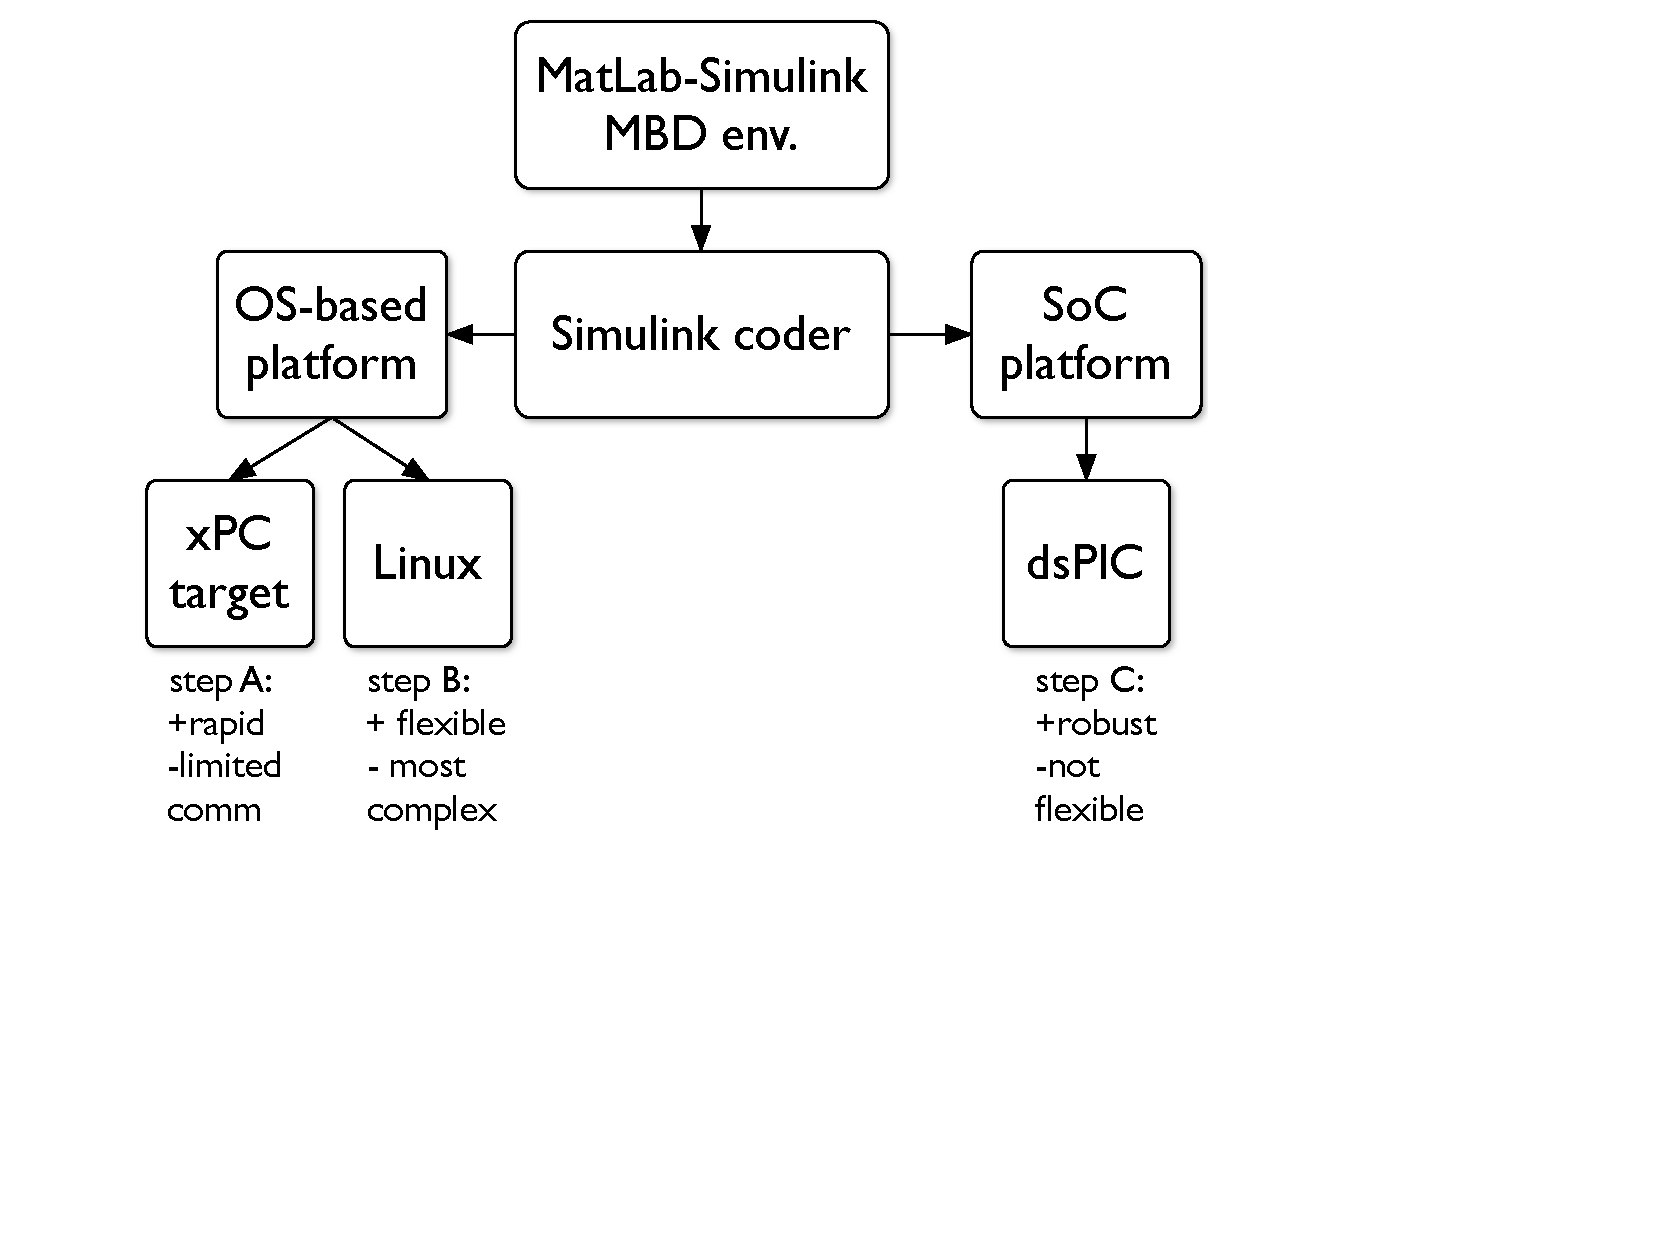
\includegraphics[width=60mm]{Pictures/Figure_001.pdf}
	\caption{Hierachy of computational platforms.}
	\label{fig:Platforms}
\end{figure}
\squeezeup
On the other hand, the specifics of R\&D work frequently require modifications of the underlying algorithms. Thus the ``xPC embedded target'' option, provided by the Simulink Coder~\cite{Simulink} is one of the best solutions  enabling frequent and rapid code modification and reintegration. An xPC target environment is a hard real-time operating system that executes the real-time code (task) that is built by the coder; the coder supports a number of computational platforms. The solution provides various services typical for an operating system while supporting preemptive mechanism  for real-time tasks scheduling and execution. The RFCPS system utilizes this option for standard \emph{Intel}x$86$ processor. While the xPC embedded target option is very flexible, it still requires ``manual'' coding in a number of occasions. Since it is hard to expect that every new piece of hardware has the same communication protocol and is supported by Mathwork's, one of the primary needs for manual coding does arise when a new communication protocol need to be implemented. Simulink coder enables integration of customized algorithms by means of s-functions; the process is time consuming, however it is well-documented and straightforward. 

The desire to focus on rapid and verifiable flight implementation of new theoretical results and well-developed legacy codes, given in a variety of programming languages, while spending less or no-time on the manual code development and re-integration resulted in targeting a new computational platform. The high computational efficiency, small footprint, rich interfacing capabilities of Linux operating system and high computational power of modern miniature computers lead to integrating this system into multiple agent flight experimentation. It is worth noting that the objectives of collaborative missions and distributed computation also require integration of messaging and synchronization mechanisms that are robust to network failures and communications dropouts. A number of industrial-grade software packages that enable communication across multiple networking nodes while explicitly addressing the messaging protocols and algorithms that are resilient to faults across local and wide area networks have been recently developed~\cite{SPREAD,MOOS}. Therefore, the most recent modification of the RFCPS included the implementation of Simulink/Coder-built algorithms along with novel messaging solutions into the Linux operating system. The capabilities of Simulink to utilize communication buses and the code defining features of the Simulink coder allow generating C/C++ libraries that are directly suitable for compilation and execution on Linux. Software API of the SPREAD toolkit~\cite{SPREAD} enables efficient messaging across various tasks executed across multiple wirelessly connected UAVs. No manual modification of the auto-generated library code is necessary, however the tasks scheduling file (main) needs to explicitly define the desired sampling rate of each of the code components and the messaging mechanism. Special consideration is given to scheduling of the flight-safety critical and not critical tasks. One of the initially developed scheduling solution utilizes a simple function call to the CPU time clock. Comparing the clock time with the required execution rate enabled efficient implementation of the required sampling of various tasks (daemons) in Linux. The most recent solution that adopts the same auto-generated code and is based on more rigorous real-time scheduling capabilities of ROS/OROCOS operating system~\cite{RosOrocos,ROS} has been also tested in the USL laboratory environment.

\subsection{RFCPS Architecture}
To enable the desired collaborative functionality the RFCPS system representing a single UAV is  comprised of the onboard and the ground segments, see Figure~\ref{fig:RFCPS_arch} .The onboard segment is built around an autopilot that brings the basic functionality of a UAV flight to the system. The current implementation of RFCPS utilizes the Piccolo series autopilots~\cite{PiccoloAP} and the corresponding ground control station that enables simultaneous operation of multiple UAVs but does not have any cooperative mission functionality built-in. 

\begin{figure}[thpb]
	\centering
	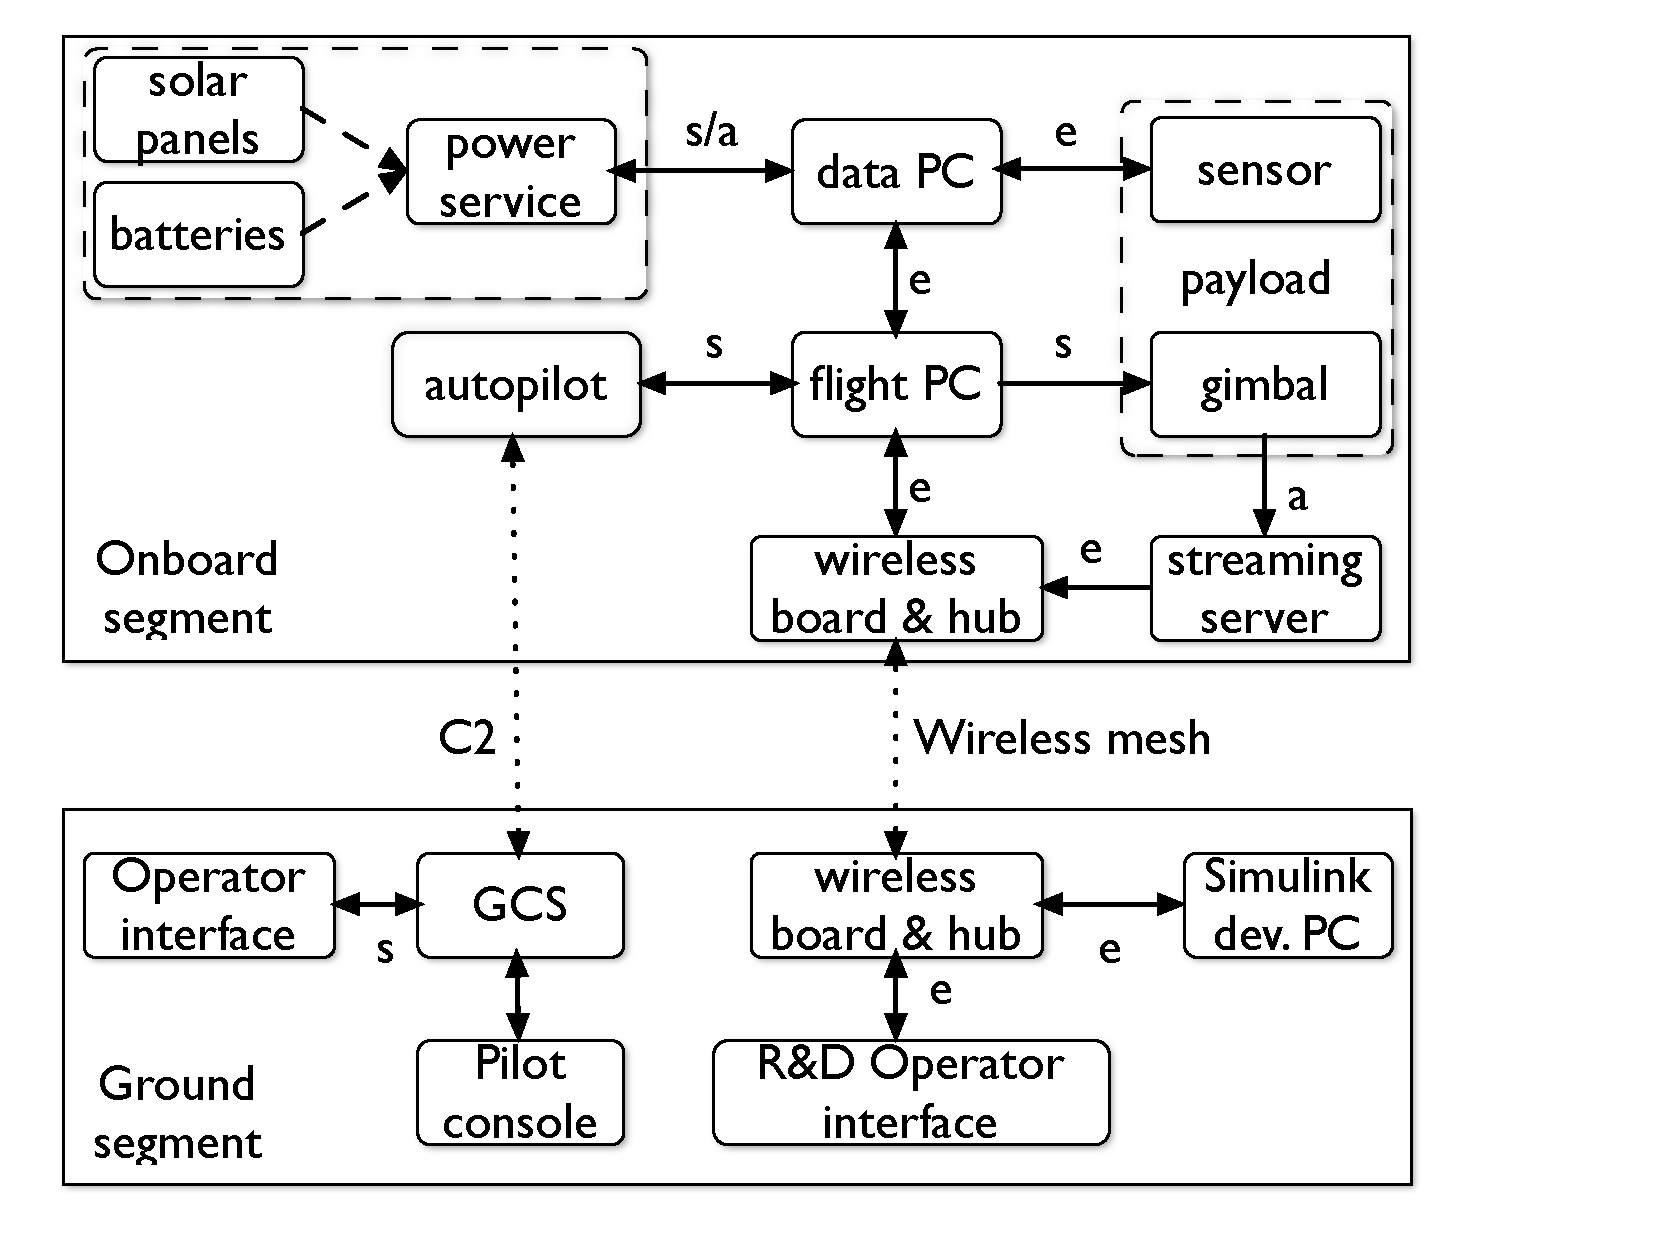
\includegraphics[width=90mm]{Pictures/Figure_02.pdf}
	\caption{Single autonomous platform as a building block of RFCPS.}
	\label{fig:RFCPS_arch}
\end{figure}
\squeezeup

The autopilot is connected over a full-duplex serial link to a flight control PC104 computer. In xPC target version, a set of communication drivers is custom-built that enable hard real-time communication with the autopilot. The drivers enable \emph{send command} and \emph{receive states} functionality and are manually coded as s-functions~\cite{DobrLizzr05}; they are automatically compiled into a binary executable file by the Simulink coder at the stage of code generation. In turn, in the Linux implementation the same drivers are given by the autopilot manufacturer. As soon as the UAV telemetry becomes available it is first used to implement the desired collaborative behavior and to control the onboard utility sensor (for example  - a high resolution camera) and its platform (gimbal); for most of the ISR missions it is common to have the imagery sensors installed on a gimbaled platform. The telemetry data is also distributed across the local onboard and the ground IP-based network for the secondary use. In particular, the data PC computer utilizes the autopilot telemetry and the utility sensor information in order to preprocess the raw data and to extract the intelligent information of interest. A very appealing feature of this data PC is that it runs a very efficient Linux operating system that enables a number of convenient services and provides very flexible access to a variety of sensors. Unlike the xPC target system, the integration of a new sensor becomes a matter of integrating a new driver that is usually provided by the sensor manufacturer, while integrating a new piece of hardware that is not supported by the xPC target is often a significant effort. As will be shown in the following chapter this data computer runs algorithms that are primarily not real time-critical and do not affect the stability and safety of UAV  flight. In the case of utilizing video cameras as ISR sensors the onboard instrumentation also contains a miniature video streaming server; although it is a single piece of hardware,  it is comprised of a frame grabber taking the analog video feed and a web server that enables live streaming of the video input into the IP-based network. Since all of the onboard components are connected over the hight speed (up to 1GigE) ethernet a number of convenient capabilities of the code development become available; some of the not flight-critical algorithms can be stopped, modified and updated while still in flight thus providing the desired flexibility for the research.

The last significant onboard component is the power management system. Depending on the specific objectives of a project it allows integrating into onboard information system a combination of solar panels and batteries. As was demonstrated in the project with autonomous cooperative thermal soaring gliders~\cite{KlassGlider}, the integration of high-output solar cells onboard enabled harvesting solar radiation thus significantly extending endurance of autonomous thermal soaring gliders. Continuos monitoring of the current state of the energy of all onboard sources enables RFCPS system to optimally plan and execute the mission.

The ground segment of RFCPS is comprised of two parts; the first part is a standalone ground control station (GCS), an operator interface (OI) computer and a command and control link provided by the autopilot manufacturer, and the second part is the research environment that is customized according to the needs of a specific mission under development. The fact that the onboard software is separated into the flight safety-critical and not flight-critical components defines the configuration of the R\&D development environment. As an example, the sensory data processing algorithms that are not flight-critical are run on a data PC; two primary OS systems are currently used - the Ubuntu Linux~\cite{Ubuntu} and ROS/OROCOS operating systems. The flight critical tasks are run under either xPC target or the ROS/OROCOS environments. Although the hardware of both PC104 computers is identical (for convenience of maintenance) the task-based separation is preserved to guarantee safety of flight experimentation and reliability of the experimental results.

To preserve the rigor of theoretical development while transitioning the results to flight the core of cooperative control algorithms is developed utilizing advanced capabilities of the Simulink environment. The Model Based Design (MBD) paradigm supported by a number of code verification and automatic code generation tools is what makes the transition very reliable. The algorithms are designed and verified in Simulink with minimal or no use of low-level programming. When debugged, the xPC target environment is used first to enable the Hardware In the Loop (HIL) simulation; Piccolo autopilot is well-supported with this functionality. Therefore, integrating and verifying the newly-built algorithms becomes straightforward; at the same time a number of data processing scripts can be built ahead of time to facilitate quick flight data analysis. After confirming the desired performance of cooperative mission in HIL setup, the same xPC based code is transformed into real-time executable and then flown. After series of flight experiments in different flight conditions the algorithms and the operational environment mature enough to allow building a set of standalone libraries for future Linux or ROS integration. The page limitation of the paper does not allow to describe all the benefits of this new direction. However note, that the same development concept is  followed and the same code that is built by the Simulink coder is used to transition the flight validated solution into a Linux/ROS based platform, see~\cite{RosOrocos} for details.

\section{Experimental Results}
To illustrate the benefits of RFCPS system that enable cooperative autonomous aerial missions this section  reviews two most recent projects. Each of these experiments highlights the key benefits of the OS-based approach.

\subsection{Coordinated Road Search by Multiple UAVs} 
The objective of this project~\cite{CPF2UAVs} was to enable a minimally trained user to utilize a number of  sensors installed onboard of heterogeneous UAVs without any need for him to be trained in flying UAVs. The concept of operation assumes that one path is generated for a number of sensors so that when they are flown autonomously the intersection of their fields of view over the sensor path is maximized. It is assumed that sensors are complementary( for example they can be electro-optical and infrared) and might have different installation onboard of UAV; body-fixed, stabilized only in roll angle or both - roll and pitch angles. Since the sensors have different degrees of freedom and the UAVs have different flight dynamic limitations, the only method of enabling the multiple sensors to coordinate their fields of view is by enabling tight cooperation of the aerial platforms. Therefore, as soon as the sensor path is extracted by the user utilizing a digital map (scribble over the map), it is submitted onboard of airborne UAVs, see Fig.~\ref{fig:CPF_concept}. 

   \begin{figure}[thpb]
      \centering
     	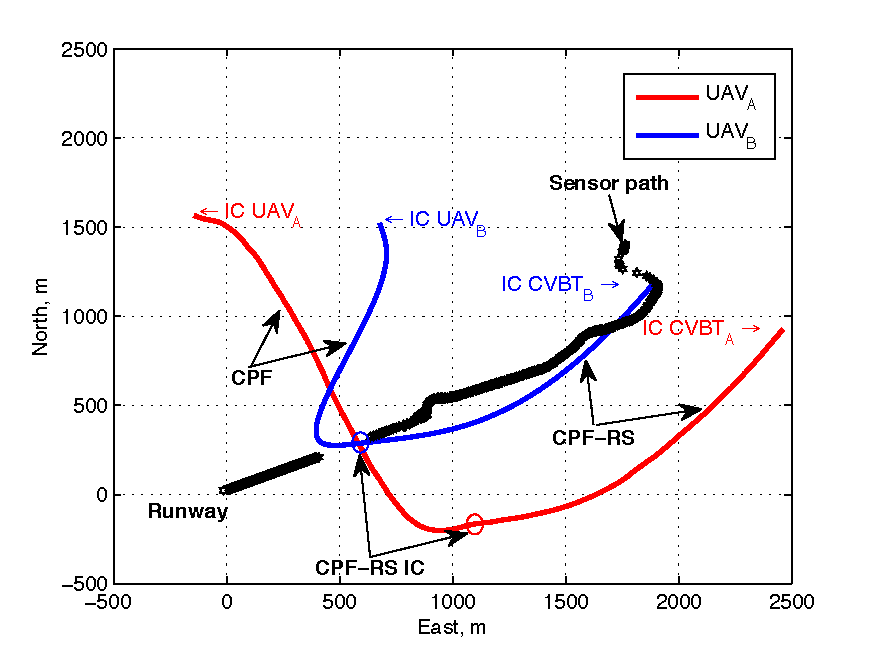
\includegraphics[scale=0.5]{Pictures/Figure_03.pdf}
      \caption{Coordinated road search mission}
      \label{fig:CPF_concept}
   \end{figure}
\squeezeup

The paths of each UAV and the desired nominal velocity profiles are then computed while accounting for the required resolution of the sensors, the UAVs flight dynamic constraints and the gimbals limitations. The UAVs are then assigned the corresponding paths with different velocity profiles to be followed in coordination (CPF); this paths define the shape of the road search (RS) segment. To execute the search the UAVs should start from their current flight state (initial conditions-IC) and perform a coordinated arrival to the beginning of the search segment. This arrival path and the velocity profiles are calculated onboard taking into account the flight dynamics  and the collision avoidance constraints.

The control~\cite{CPF2UAVs} that is implemented by each UAV during the mission is based on the explicit separation of time and space. The  path is parameterized by algebraic polynomials, therefore the number of parameters defining the path is finite and depends on the class and the degree of the chosen polynomial representation. Supported by robust communication protocols this approach enables feasible real-time execution, path generation and simple and inexpensive communication of the intent and current state of each UAV that is critical especially for the collision avoidance, see Fig.~\ref{fig:CPF}.
   \begin{figure}[thpb]
      \centering
      %\framebox{\parbox{3in}{Control architecture of the cooperative mission.}}
      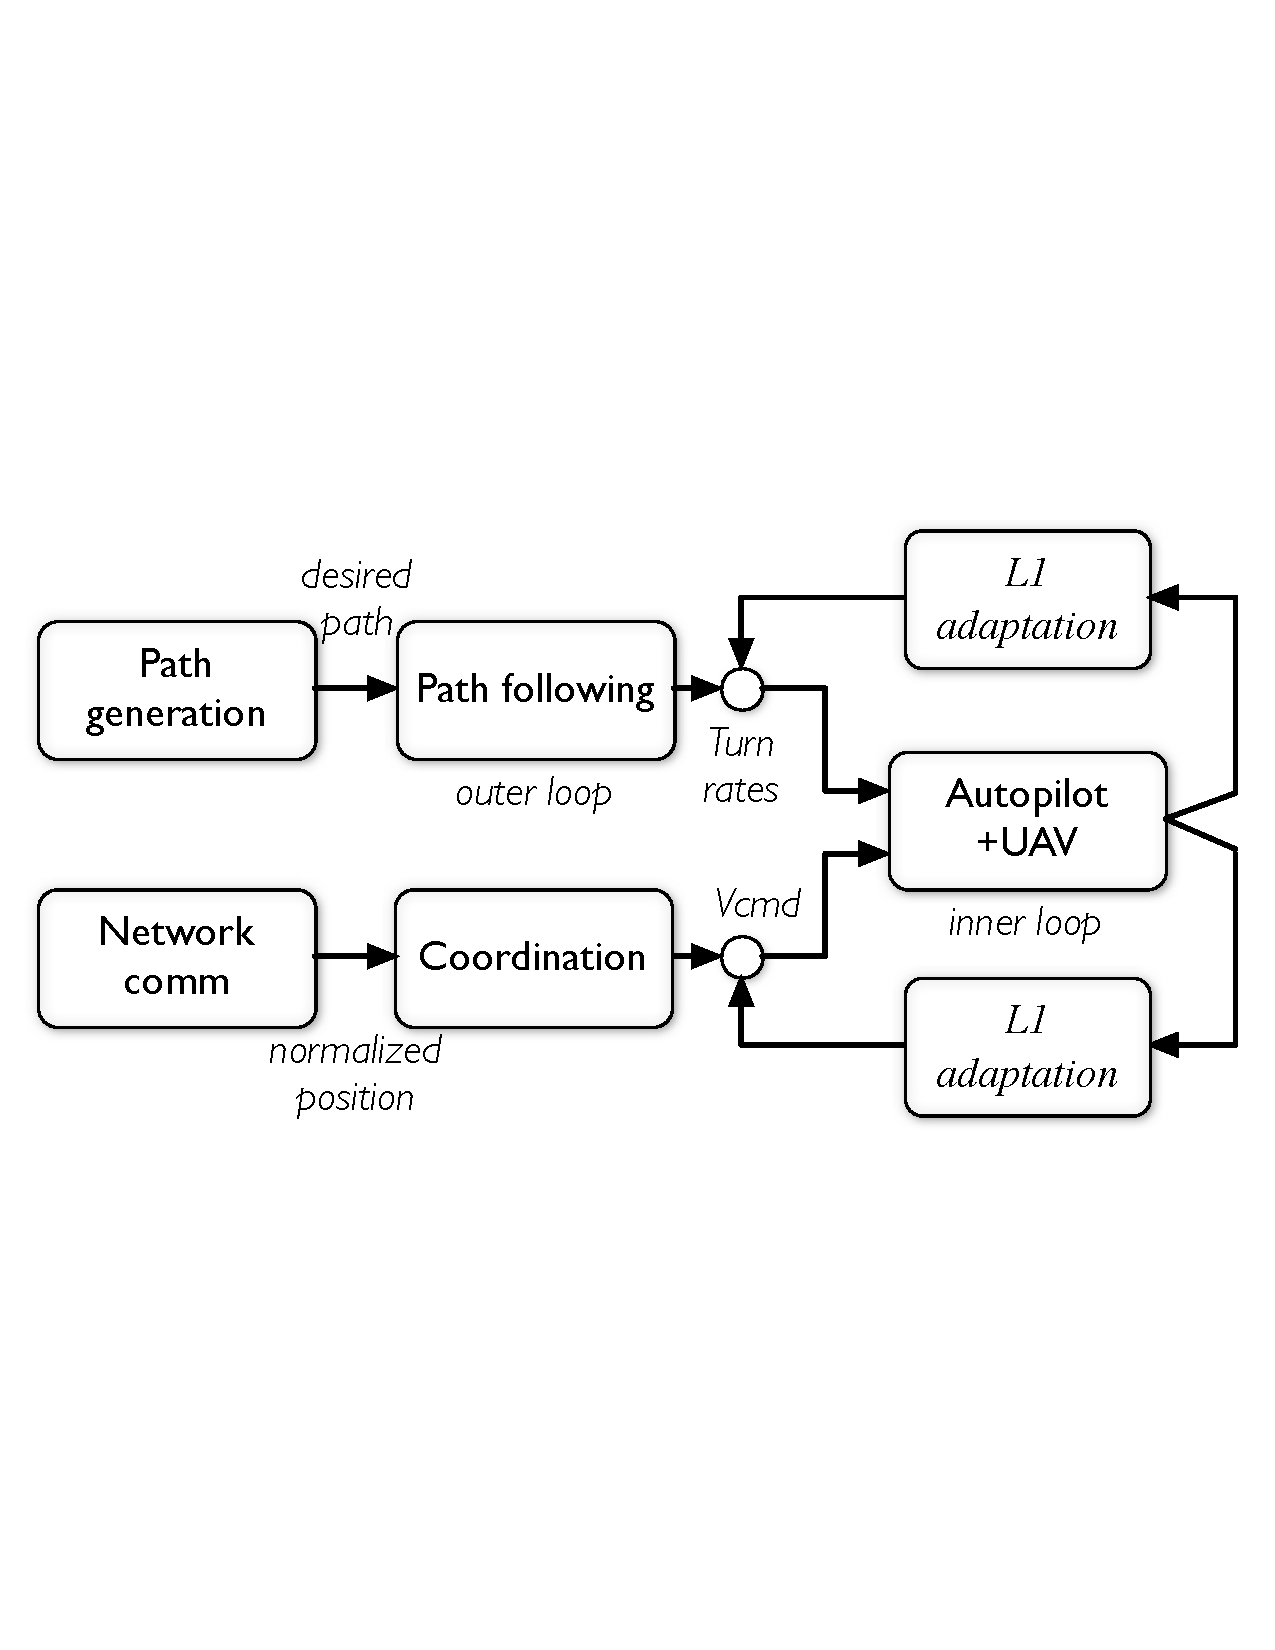
\includegraphics[width=70mm]{Pictures/Figure_04.pdf}
      \caption{Control architecture of the cooperative mission}
      \label{fig:CPF}
   \end{figure}
\squeezeup
 The path following control~\cite{CPF2UAVs} for fixed wing UAVs is enabled by using attitude control commands: pitch and yaw rates are the primary control signals utilized by the nonlinear control law. If the UAVs were following the assigned path and the velocity profiles precisely then there would not be any need for tight flight coordination; the coordination is already accounted at the stage of the path and velocity profile generation. However each UAV is subject to numerous disturbances resulting in the path following and coordination errors. To provide close coordination the velocity of each UAV is used to minimize a so-called coordination error that is calculated onboard of each UAV based on the exchange of coordination states by all airborne vehicles over the wireless mesh network. The developed algorithm is robust to network dropouts and allows tight coordination of a number of UAVs flying in a realistic environment. Besides the coordination and path following algorithms the onboard flight-critical computer runs the  $L_1$ adaptive control law implemented as an output feedback augmentation loop around the nominal autopilot; the overall coordinated path following control architecture is presented in Fig.~\ref{fig:CPF}.  Implementing the $L_1$ adaptive controller onboard provides guaranteed performance of the entire fleet of UAVs in a wide range of operational conditions with no need for retuning of the individual systems component, an interested reader is referred to~\cite{L1CPF} for more details.

The desired performance of airborne sensors in this scenario is enabled by the ability to execute onboard the path following and coordination algorithms in hard real-time and the imagery and video processing tasks executed as non real-time critical processes. Furthermore, while transmitting the overlapped video and imagery over the wireless network, the data pre-processing algorithms  solve a number of typical tasks such as extraction of objects of interest (cars, people, buildings e.t.c) and their geo-referencing. Therefore, by enabling coordination not only the content of sensory data becomes rich and meaningful but the operator is alerted when an object of interest is detected. The overall load of the operator thus is significantly lower. 

\subsection{Cognitive Automation in Support of Mission Planning and Execution} 

The objective of this project was to assist a single operator in designing and executing a multiple UAV mission by combining the high-level mission planning algorithms with cooperative path following of a number of UAVs. As a first step in achieving this goal the project concentrated on a single UAV mission with the rest of the fleet being modeled on the ground. 

Therefore, the CoCAMPUS (Cooperative Cognitive Automation through Mathematically Optimized Path-Following of UAVs) project~\cite{COSA2} was conducted to explore how to achieve project objectives. A typical mission was chosen based on a simplified air-attack scenario that also included static threats at unknown locations; it was assumed that the UAVs will discover the static surface to air missile (SAM) sites during the mission execution. The Cognitive System Architecture (COSA2)~\cite{COSA2} was integrated onboard  to implement cognitive behavior on the basis of current understanding of tactical situation and explicit knowledge models,  while deriving implicit cost-functions and defining the path optimization constraints during the flight.

Artificial Cognitive Units (ACUs) onboard the UAV are used to implement task-based guidance and mimic human rationality to some extent, forming so-called cognitive automation, processing information mostly on a symbolic level. The ACU behavior is completely defined by its goal, which is explicitly represented as knowledge in its implementation.The ACU allows implementation of knowledge-based algorithms such as decision making and planning that depend on the available tactical observations and understanding of the current situation. It also offers semi-autonomous capabilities, in a sense that the ACU pursues a task autonomously using the automation built inside the UAV system.

The objective of a single human operator in the air-attack mission is to perform a combat air patrol (CAP) and, upon detection of a ground vehicle and its identification, to approach and attack the target. The no-fly zones and the static threats in form of SAM-sites are to be avoided as they are detected. The ground target is located on a road inside the mission area and its coordinates are given by an external reconnaissance system cooperating with the operator. The final approach to the target by a UAV should be performed at an optimal course providing the highest effectiveness of released material; during the flight the effectiveness was evaluated by taking a picture at the calculated release point and analyzing if the target was present in the camera frame. 

Figure~\ref{fig:CAP_mission} presents the mission progress during the CoCAMPUS flight trials. The flight path can be separated into two consecutive segments. First, the operator chose and commanded the desired CAP (CAP A) to the ACU in point 1. Upon arriving and orbiting at the CAP (point 2) and reevaluating the situation, the operator tasked the ACU to attack the ground vehicle. The UAV started the task by dynamically calculating an optimal approach to the road (point 3) before attacking the target vehicle in point 4. Upon taking a picture, the ACU commanded to circle the target position for further damage assessment. At all times during the mission, the ACU monitored the UAV systems and flight states and matched them with its own projection of future environment states, to ensure the fulfillment of the task-queue and possibly counteract aberrations. The path generation module took into account all given threats and dynamic constraints to ensure a safe, feasible path and to allow the best approach to the target.

   \begin{figure}[thpb]
      \centering
      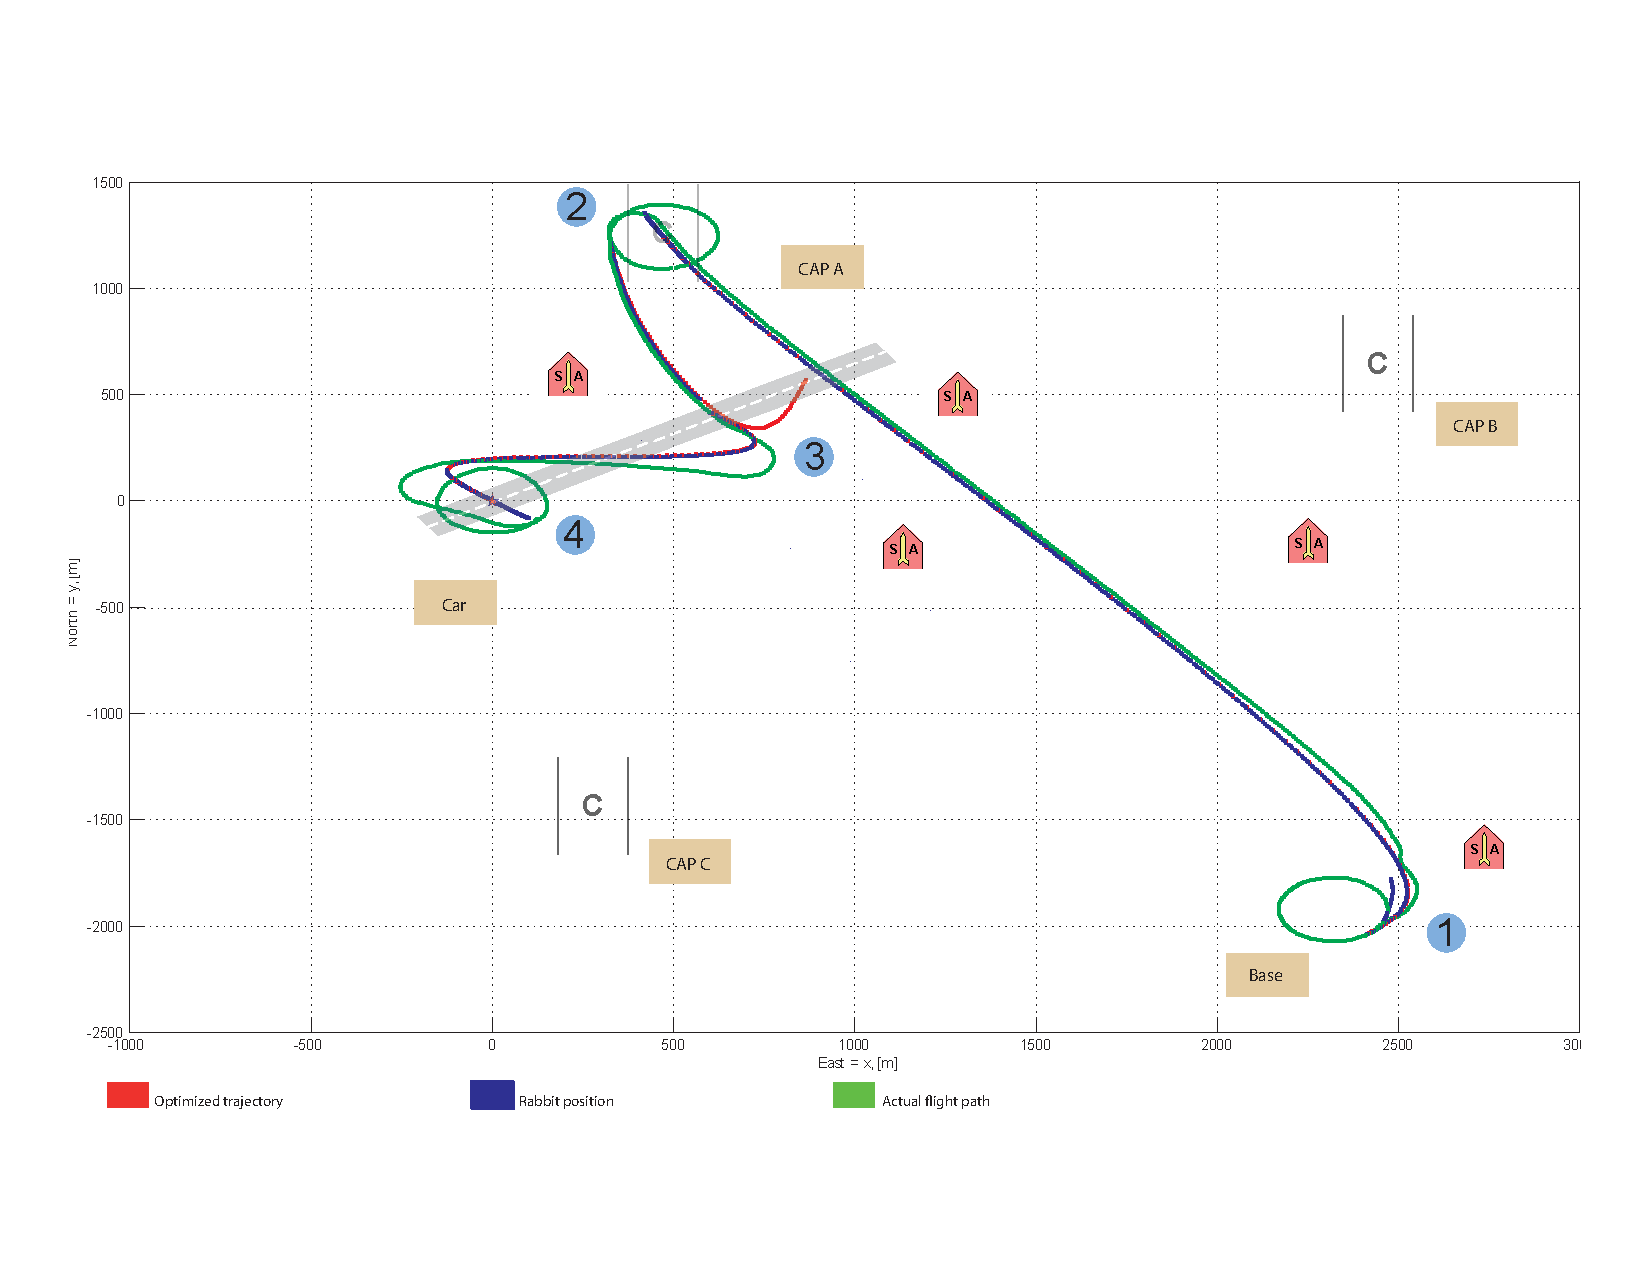
\includegraphics[width=87mm]{Pictures/CAP_mission.pdf}
      \caption{Air-Attack mission results with overlaid tactical elements.}
      \label{fig:CAP_mission}
   \end{figure}
\squeezeup

The tasks of cognitive automation as well as flight critical control have been implemented onboard of single CPU running Linux operating system. The coordinated path following task has been designed in Simulink and the code was auto-generated and recompiled in Linux. The flight control law was manually scheduled at $100 Hz$ rate while the communication with autopilot run at $50 Hz$. The COSA2 tasks were running natively in Linux as background processes.

Flight tests were performed over multiple days and have consistently shown verifiable and repeatable results. These real-world operational flight trials have proven the feasibility and the benefits of the presented approach and the developed hardware architecture. The goal-driven ACU enhances the system robustness in mission execution and supports the human operator, resulting in a significantly reduced workload.

\subsection{Conclusion}
The paper presented the evolution of the RFCPS system that address the cooperative missions of multiple UAVs. The design of the RFCPS is driven by the mission level objectives and is enabled on the one hand by the progress in miniature sensors, computational power, communication and portable energy technologies and on the other hand by the advanced capabilities of embedded control and communication oriented software. As a result, the RFCPS enables rapid "prototyping of cooperative mission" of multiple UAVs that seemed impossible just a couple of years ago. 

\addtolength{\textheight}{-15.5cm}   % This command serves to balance the column lengths
                                  % on the last page of the document manually. It shortens
                                  % the textheight of the last page by a suitable amount.
                                  % This command does not take effect until the next page
                                  % so it should come on the page before the last. Make
                                  % sure that you do not shorten the textheight too much.

%%%%%%%%%%%%%%%%%%%%%%%%%%%%%%%%%%%%%%%%%%%%%%%%%%%%%%%%%%%%%%%%%%%%%%%%%%%%%%%%

\section*{ACKNOWLEDGMENT}

Evolution of RFCPS system has been funded in part by the National Air and Space Administration under Contracts NNX08BA64A, NNX08BA65A, NNX08AB97A, NNX08AC81A, and NNL08AA12I; ARO under Contract No.W911NF-06-1-0330, the USSOCOM/NPS Field Experimentation Cooperative, the Office of Naval Research under Contract N00014-05-1-0828. 

%%%%%%%%%%%%%%%%%%%%%%%%%%%%%%%%%%%%%%%%%%%%%%%%%%%%%%%%%%%%%%%%%%%%%%%%%%%%%%%%

\begin{thebibliography}{99}

\bibitem{SOTECH2012} H., Canaday, UAV Payload Systems, in Special Operations Technology, Vol.10, Issue 6, 2012.
\bibitem{DefInd2010} ``Too Much Information: Taming the UAV Data Explosion,'' in Defense Industry Daily, May 16, 2010.
\bibitem{Stevens08} R.C., Stevens, S.A., Firooz, J.R., Braegelmann, A.M., Cordes, R.L., Nelson, Small unmanned aerial vehicle (UAV) real-time intelligence, surveillance, and reconnaissance (ISR) using onboard pre-processing, in proceedings  of the XVIII SPIE Congress on Automatic Target Recognition, vol. 6967, pp. 696717-696717-8, 2008.
\bibitem{Simulink} MathWork's Simulink/Coder, http://www.mathworks.com/ products/simulink/, last accessed on 09/20/12.
\bibitem{SLUGap09} M., Lizarraga, G.H., Elkaim, G., Horn, R., Curry, V.N., Dobrokhodov, I.I., Kaminer, Low Cost Rapidly Reconfigurable UAV Autopilot for Research and Development of Guidance, Navigation and Control Algorithms, in proceedings of ASME/IEEE MESA09, International Conference on Mechatronic and Embedded Systems and Applications, San Diego, August, 2009.
\bibitem{SLUGarch2011} M., Lizarraga, R., Curry, G.H., Elkaim, Reprogrammable UAV Autopilot System (Part 1) - System Hardware and Software, in Circuit Cellar, Issue 249, April 2011.
\bibitem{SLUGtest2011} M., Lizarraga, R., Curry, G.H., Elkaim, Reprogrammable UAV Autopilot System (Part 1) - testing and Results, in Circuit Cellar, Issue 250, May 2011.
\bibitem{SPREAD} The Spread Toolkit, http://www.spread.org, last accessed on 09/20/12.
\bibitem{MOOS} The MOOS Software, http://www.robots.ox.ac.uk/, last accessed on 09/20/12.
\bibitem{RosOrocos} The OROCOS Project, http://www.orocos.org, last accessed on 09/20/12.
\bibitem{ROS} Robotic Operating System, http://www.ros.org, last accessed on 09/20/12.
\bibitem{PiccoloAP} Piccolo Autopilots, http://www.cloudcaptech.com, last accessed on 09/20/12.
\bibitem{DobrLizzr05} V.N., Dobrokhodov, M., Lizarraga, Developing Serial Communication Interfaces for Rapid Prototyping of Navigation and Control Tasks, in proceedings of AIAA Modeling and Simulation Technologies Conference and Exhibit, pp13, 2005.
\bibitem{Ubuntu} UBUNTU Operating System, http://www.ubuntu.com, last accessed on 09/20/12.
\bibitem{KlassGlider} K., Andersson, K.D., Jones, V.N., Dobrokhodov, I.I., Kaminer, Thermal Highs and Pitfall Lows. Notes on the Journey to the First Cooperative Autonomous Soaring Flight, 51st IEEE Conference on Decision and Control, Maui, Hawaii, December 10-13, 2012.
\bibitem{CPF2UAVs} E., Xargay, V.N., Dobrokhodov, I.I., Kaminer, A.M., Pascoal, N., Hovakimyan, and C., Cao, �Time�Coordinated Path Following of Multiple Heterogeneous Vehicles over Time�Varying Networks,�  IEEE Control Systems Magazine, Special Issue on UAVs and Controls, 2012.
\bibitem{L1CPF} I.I., Kaminer, A.M., Pascoal, E., Xargay, C. Cao, N., Hovakimyan, V.N., Dobrokhodov, �3D Path Following for Small UAVs using Commercial Autopilots augmented by L1 Adaptive Control,� Journal of Guidance, Control, and Dynamics, N 0731-5090 vol.33 no.2 (550-564) 2010.
\bibitem{COSA2} S., Clauss, P.,  Aurich, S.,  Br�ggenwirth, V.N., Dobrokhodov, I.I., Kaminer, A., Schulte: "Design and Evaluation of a UAS combining Cognitive Automation and Optimal Control", Infotech@Aerospace 2012, Garden Grove, California, June 19-21, 2012.
\end{thebibliography}
\end{document}
